\documentclass[letterpaper]{article}
\usepackage[utf8]{inputenc}
\usepackage[parfill]{parskip}    % Activate to begin paragraphs with an empty line rather than an indent
\usepackage{graphicx}
\usepackage{amssymb}
\usepackage{amsmath}
\usepackage{amsthm}
\usepackage{mathtools}
\usepackage{mathrsfs}

\usepackage{afterpage}

\usepackage{algorithm}
\usepackage{algpseudocode}

\usepackage{verse}

\newtheorem{theorem}{Theorem}[section]
\newtheorem{corollary}{Corollary}[theorem]
\newtheorem{lemma}[theorem]{Lemma}

\theoremstyle{remark}
\newtheorem*{remark}{Remark}

\usepackage{epstopdf}
\usepackage{circuitikz}
\usetikzlibrary{angles, quotes}
\usepackage[separate-uncertainty = true,multi-part-units=single]{siunitx}
\usepackage{booktabs}
\usepackage{enumitem}
\usepackage[toc,page]{appendix}
\usepackage{color}
\usepackage{pgfplots}
\usepackage{pgfplotstable}
\usepackage{caption}
\usepackage{subcaption}
\usepackage{url}
\usepackage{multirow}
\usepackage{makecell}
\usepackage[round]{natbib}   % omit 'round' option if you prefer square brackets
\usepackage{titling}
\usepackage{siunitx}
\usepackage{physics}

\usepackage{setspace}
% \doublespacing
\usepackage{float}


\pgfplotsset{compat=1.14}

%  Special math symbols
%       floor, ceiling, angled brackets
%-----------------------------------------------------------------------
\newcommand{\floor}[1]{\left\lfloor #1\right\rfloor}
\newcommand{\ceil}[1]{\left\lceil #1\right\rceil}
\newcommand{\etal}{\textit{et al.}}
\newcommand{\RE}{\mathbb{R}}        % real space
\newcommand{\ZZ}{\mathbb{Z}}        % integers
\newcommand{\NN}{\mathbb{N}}        % natural numbers
\newcommand{\eps}{{\varepsilon}}    % prettier epsilon
%-----------------------------------------------------------------------
%  Tighter lists
%-----------------------------------------------------------------------
\newenvironment{itemize*}% Tighter itemized list
  {\begin{itemize}%
    \setlength{\itemsep}{-0.5ex}%
    \setlength{\parsep}{0pt}}%
  {\end{itemize}}
\newenvironment{description*}% Tighter description list
  {\begin{description}%
    \setlength{\itemsep}{-0.5ex}%
    \setlength{\parsep}{0pt}}%
  {\end{description}}
\newenvironment{enumerate*}% Tighter enumerated list
  {\begin{enumerate}%
    \setlength{\itemsep}{-0.5ex}%
    \setlength{\parsep}{0pt}}%
  {\end{enumerate}}
%-----------------------------------------------------------------------
% Typing shortcuts
%-----------------------------------------------------------------------
\newcommand{\X}{\mathbb{X}}
\newcommand{\SG}{\mathbf{S}}
\newcommand{\GE}{\mathcal{G}}
\newcommand{\ST}{\,:\,}
\renewcommand{\tilde}[1]{\widetilde{#1}}
\newcommand{\diam}{\mathrm{diam}}
\newcommand{\sq}{\square}
\newcommand{\half}[1]{\frac{#1}{2}}
\newcommand{\inv}[1]{\frac{1}{#1}}
\newcommand{\alg}{\textsf{SplitReduce}}
\newcommand{\sz}[1]{\sigma_{#1}}
\newcommand{\LL}{\mathcal{L}}
\newcommand{\softOmega}{\widetilde{\Omega}} 
\newcommand{\softO}{\widetilde{O}}
\newcommand{\OO}{O^*}  %or \widetilde{O}?

\newcommand{\Null}[1]{\text{Null}(#1)}


\newcommand{\dx}{\mathrm{d}x}
\newcommand{\dy}{\mathrm{d}y}
\newcommand{\dz}{\mathrm{d}z}
\newcommand{\dt}{\mathrm{d}t}
\newcommand{\du}{\mathrm{d}u}
\newcommand{\dtheta}{\mathrm{d}\theta}
\newcommand{\dq}{\mathrm{d}q}
\newcommand{\diff}{\mathrm{d}}
\newcommand{\dV}{\mathrm{d}V}
\newcommand{\dL}{\mathrm{d}L}
\newcommand{\dA}{\mathrm{d}A}
\newcommand{\dH}{\mathrm{d}H}
\newcommand{\df}{\mathrm{d}f}
\newcommand{\dg}{\mathrm{d}g}
\newcommand{\dr}{\mathrm{d}r}
\newcommand{\dw}{\mathrm{d}w}
\newcommand{\dI}{\mathrm{d}I}

\newcommand*\len[1]{\overline{#1}}


\newcommand\note[1]{\marginpar{\textcolor{red}{#1}}}
\newcommand*{\tageq}{\refstepcounter{equation}\tag{\theequation}}

\newcommand*{\equals}{=}

\usepackage{fancyhdr}

\pgfplotscreateplotcyclelist{grayscale}{
    thick,white!10!black,mark=x,mark options=solid, dashed\\%
    thick,white!20!black,mark=o,mark options=solid\\%
}

\newcommand{\mat}[1]{\ensuremath{\begin{bmatrix}#1\end{bmatrix}}}
\newcommand{\cat}[1]{\ensuremath{\begin{vmatrix}#1\end{vmatrix}}}
\newcommand{\eqn}[1]{\begin{alignat*}{2}#1\end{alignat*}}
\newcommand{\p}[2]{\frac{\partial #1}{\partial #2}}
\newcommand*{\thus}{&\implies\quad&}

\newcommand{\answer}[1]{\framebox{$\displaystyle #1 $}}

\newcommand{\shrug}[1][]{%
\begin{tikzpicture}[baseline,x=0.8\ht\strutbox,y=0.8\ht\strutbox,line width=0.125ex,#1]
\def\arm{(-2.5,0.95) to (-2,0.95) (-1.9,1) to (-1.5,0) (-1.35,0) to (-0.8,0)};
\draw \arm;
\draw[xscale=-1] \arm;
\def\headpart{(0.6,0) arc[start angle=-40, end angle=40,x radius=0.6,y radius=0.8]};
\draw \headpart;
\draw[xscale=-1] \headpart;
\def\eye{(-0.075,0.15) .. controls (0.02,0) .. (0.075,-0.15)};
\draw[shift={(-0.3,0.8)}] \eye;
\draw[shift={(0,0.85)}] \eye;
% draw mouth
\draw (-0.1,0.2) to [out=15,in=-100] (0.4,0.95); 
\end{tikzpicture}}


\pagestyle{fancy}
\fancyhf{}
\rhead{Rahul Arya}
\lhead{EE 16B}
\cfoot{\thepage}

\title{Lecture 26 - Notes}
\author{Rahul Arya}
\date{April 2019}
\begin{document}

\maketitle

\section{Overview}
In previous lectures, we explored various properties of the DFT matrix $F_N$. Now, we will look at how this matrix can be used to rewrite a discrete-time signal in the frequency domain, by considering the vector $\vec{X} = F_N\vec{x}$ where $\vec{x}$ is a discrete-time signal of length $N$. In particular, we claim that the vector $\vec{X} = F_N\vec{x}$ will represent coefficients of sinusoids that, when summed and sampled at fixed intervals, will equal the original $\vec{x}$.

\section{Identifying a Single Sinusoid}
To look at even a simple example of the DFT, we must first remind ourselves what a discrete-time signal represents. Recall that a discrete-time signal represents \emph{samples} of a continuous-time signal, made every $\Delta$ time steps. So, if a continuous signal $x(t)$ is converted into a discrete-time signal $\vec{x}$, we have that
\[
    x(k\Delta) = \vec{x}[k]
\]
for integers $k$.

Thus, if our discrete-time signal $\vec{x}$ has length $N$, it can be thought of as samples made of an unknown continuous time signal with duration $T = N\Delta$. It is natural to consider all the periodic sinusoids over this duration, since we will use them to form our basis in the frequency domain. The most obvious sinusoid to consider is the one with time period $T$ and frequency $f_0 = 1 / T$. Plotting this sinusoid, we obtain:
\begin{center}
\begin{tikzpicture}
\begin{axis}[
    xlabel=$t / T$, ylabel=$ $,
    xmin=0, xmax=1,
    ymin=-1.2, ymax=1.2,
    legend style={at={(1.02,1)},anchor=north west},
 ]
\addplot [domain=0:1, samples=100] {cos(360 * x)};
\addlegendentry{$\cos(2\pi f_0 t)$};
\end{axis}
\end{tikzpicture}
\end{center}
This sinusoid is known as the \emph{first harmonic} of our sampling period, with $f_0$ known as the \emph{fundamental frequency}. It is clear that by choosing frequencies that are integer multiples of $f_0$, we will obtain more signals that are periodic in time $T$, as shown:
\begin{center}
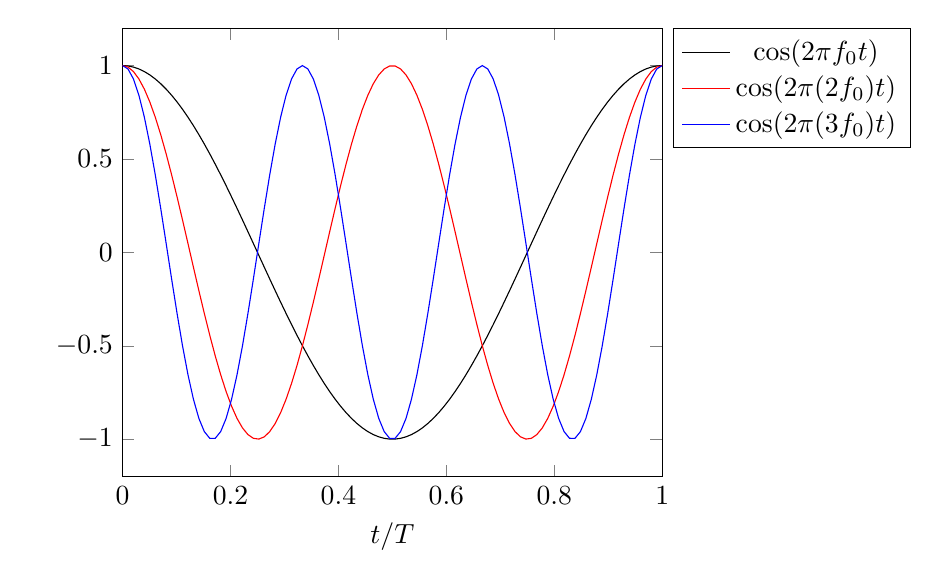
\begin{tikzpicture}
\begin{axis}[
    xlabel=$t / T$, ylabel=$ $,
    xmin=0, xmax=1,
    ymin=-1.2, ymax=1.2,
    legend style={at={(1.02,1)},anchor=north west},
 ]
\addplot [domain=0:1, samples=100] {cos(360 * x)};
\addlegendentry{$\cos(2\pi f_0 t)$};
\addplot [domain=0:1, samples=100, red] {cos(2 * 360 * x)};
\addlegendentry{$\cos(2\pi (2f_0) t)$};
\addplot [domain=0:1, samples=100, blue] {cos(3 * 360 * x)};
\addlegendentry{$\cos(2\pi (3f_0) t)$};
\end{axis}
\end{tikzpicture}
\end{center}
These signals are known as the 2nd and 3rd harmonics.

In a similar manner, the $l$th harmonic is a sinusoidal signal that has $l$ periods over the interval $T$. Consider the general equation of the $l$th harmonic with amplitude $A_l$ and phase shift $\phi_l$, so
\[
    x(t) = A_l\cos(2\pi (lf_0) t + \phi_l).
\]
After sampling this sinusoid at $N$ points, we obtain the discrete-time signal represented by the points on the following graph:
\begin{center}
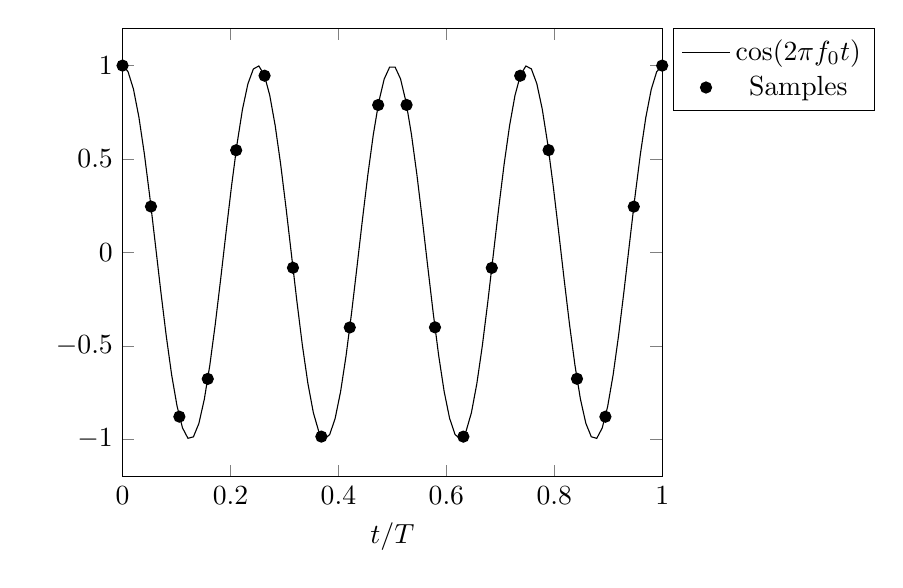
\begin{tikzpicture}
\begin{axis}[
    xlabel=$t / T$, ylabel=$ $,
    xmin=0, xmax=1,
    ymin=-1.2, ymax=1.2,
    legend style={at={(1.02,1)},anchor=north west},
 ]
\addplot [domain=0:1, samples=100] {cos(4*360 * x)};
\addlegendentry{$\cos(2\pi f_0 t)$};
\addplot [domain=0:1, samples=100, samples=20, mark options = {black}, only marks] {cos(4*360 * x)};
\addlegendentry{Samples};
% \addplot [domain=10^(-2):1] {x};
% \addplot [domain=1:10^(2)] {1 / x};
% \addlegendentry{Approximation};
\end{axis}
\end{tikzpicture}
\end{center}
Expressed symbolically as a vector $\vec{x}$, it is clear that its $k$th component
\[
    \vec{x}[k] = A_l\cos(2\pi (lf_0) k\Delta + \phi_l),
\]
since after $k$ samples $t = k\Delta$. Substituting in our known values for $f_0$ and $\Delta$ in terms of $N$ and $T$, we obtain
\eqn{
    && \vec{x}[k] &= A_l\cos(2\pi lf_0 k\Delta + \phi_l) \\
    &&&= A_l\cos(2\pi \frac{1}{T} lk \frac{T}{N} + \phi_l) \\
    &&&= A_l\cos(\frac{2\pi lk}{N} + \phi_l),
}
for all integers $0 \le k < N$.

Now we know what our discrete-time signal $\vec{x}$ looks like, we can turn our attention towards computing $F_N\vec{x}$. However, notice that $F_N$ is defined using complex numbers written in polar form, where their arguments represent the phase. It would be nice to write each component of $\vec{x}$ in a similar manner, to make computing and evaluating $F_N\vec{x}$ easier. Of course, we have done something very similar before, when we wrote sinusoidal functions as phasors back in Module 1. In an exactly analogous manner, we can express
\eqn{
    && \vec{x}[k] &= A_l\cos(\frac{2\pi lk}{N} + \phi_l) \\
    &&&= \frac{A_l}{2} \left( e^{2\pi jlk / N} e^{j\phi_l} + e^{-2\pi j lk / N} e^{-j\phi_l} \right) \\
    &&&= \frac{1}{2} (A_le^{j\phi_l}\omega_N^{lk} + \overline{A_le^{j\phi_l}}\omega_N^{-lk} ).
}
pulling the root of unity $\omega_N$ out from the exponential terms. For notational convenience, let $C_l = A_le^{j\phi_l}$. In some sense, we can think of $C_l$ as the ``phasor'' representation of our signal.

Recall that we defined the $\vec{u}_l$ to be the columns (or rows, since $F_N$ is symmetric) of $F_N$. Observe in particular that we can rewrite the above expression as
\eqn{
    && \vec{x}[k] &= \frac{1}{2} (C_l\omega_N^{lk} + \overline{C_l}\omega_N^{-lk}) \\
    &&&= \frac{1}{2} (C_l\omega_N^{(l - lN)k} + \overline{C_l}\omega_N^{-lk}) \\
    &&&= \frac{1}{2} (C_l\omega_N^{-(N - 1)lk} + \overline{C_l}\omega_N^{-lk}),
}
since $\omega_N^N = 1$, so we have that
\[
    \vec{x} = \frac{1}{2} (C_l\vec{u}_l e^{j\phi_l} + \overline{C_l}\vec{u}_{N - l} e^{-j\phi_l}) = \frac{1}{2} (C_l\overline{\vec{u}_l} e^{j\phi_l} + \overline{C_l}\overline{\vec{u}_{N-l}} e^{-j\phi_l}),
\]
since we saw last time that $\vec{u}_l$ and $\vec{u}_{N-l}$ were complex conjugates of one another.

Now, we can finally evaluate $F_N\vec{x}$ directly, to obtain
\eqn{
    && X &= F_N \vec{x} \\
    &&&= \frac{1}{2} F_N (C_l\overline{\vec{u}_l} e^{j\phi_l} + \overline{C_l}\overline{\vec{u}_{N-l}} e^{-j\phi_l}) \\
    &&&= \frac{1}{2} \mat{ - & \vec{u}_0^T & - \\ & \vdots & \\ - & \vec{u}_{N-1}^T & - } (C_l\overline{\vec{u}_l} + \overline{C_l}\overline{\vec{u}_{N-l}}) \\
    &&&= \frac{C_l}{2} \mat{ - & \vec{u}_0^T & - \\ & \vdots & \\ - & \vec{u}_{N-1}^T & - } \overline{\vec{u}_l} + \frac{\overline{C_l}}{2} \mat{ - & \vec{u}_0^T & - \\ & \vdots & \\ - & \vec{u}_{N-1}^T & - } \overline{\vec{u}_{N-l}} \\
    &&&= \frac{C_l}{2} \mat{ \vec{u}_0^T\overline{\vec{u}_l} \\ \vdots \\ \vec{u}_{N-1}^T\overline{\vec{u}_l}} + \frac{\overline{C_l}}{2} \mat{ \vec{u}_0^T\overline{\vec{u}_{N - l}} \\ \vdots \\ \vec{u}_{N-1}^T\overline{\vec{u}_{N - l}}} \\
    &&&= \frac{C_l}{2} \mat{\langle \vec{u}_0, \vec{u}_l \rangle \\ \vdots \\ \langle \vec{u}_{N-1}, \vec{u}_l \rangle} + \frac{\overline{C_l}}{2} \mat{\langle \vec{u}_0, \vec{u}_{N-l} \rangle \\ \vdots \\ \langle \vec{u}_{N-1}, \vec{u}_{N-l} \rangle}.
}
Recall from last lecture that all the $\vec{u}_i$ were mutually orthogonal and each had norm $\sqrt{N}$. Thus, we can evaluate all the above inner products, to finally obtain
\eqn{
    && X &= \frac{C_l}{2} \mat{0 \\ \vdots \\ N \\ \vdots \\ 0 \\ \vdots \\ 0} + \frac{\overline{C_l}}{2} \mat{0 \\ \vdots \\ 0 \\ \vdots \\ N \\ \vdots \\ 0} = \frac{N}{2} \mat{0 \\ \vdots \\ C_l \\ \vdots \\ \overline{C_l} \\ \vdots \\ 0},
}
where the nonzero entries lie at indices $l$ and $N - l$, respectively.

This seems interesting. By looking at the positions of the nonzero components of $X$, we can determine the frequency $lf_0$ of the original signal, and by looking ath the magnitude and phase of the nonzero entry $C_l$, we can compute the magnitude and phase of the original signal. 

In other words, starting with discrete-time samples of a continuous sinusoid with frequency $lf_0$, amplitude $A_l$, and phase shift $\phi_l$, we could apply the DFT to obtain a sparse vector from which we can easily read off the key properties of our original signal!

So for what $l$ does this approach work? Notice that for sufficiently large $l$, the top and bottom terms (i.e. the terms at indices $l$ and $N-l$) will collide and then overlap, meaning that we may not be able to determine the frequency of our original signal - in fact, our original signal may appear like another signal of a much lower frequency! This phenomenon is known as \emph{aliasing}, and can be taken into account in some contexts to recover the original signal anyway. 

However, we will not study it in great detail here, focusing on the simpler case where the two terms do not overlap. Some simple arithmetic shows that, if we wish to accommodate frequencies up to $Mf_0$ for some integer $M$, we will need at least $N = 2M + 1$ samples to ensure that the two terms do not overlap.

\section{Identifying a Superposition of Sinusoids}
Of course, it is rarely the case that we are given samples of a single sinusoid and asked to identify its characteristics. Rather, in applications such as audio processing, we may be provided with samples of a signal consisting of the superposition of many different harmonics, and be asked to write the signal as a linear combination of all these harmonics. More precisely, let our received signal be
\[
    \vec{x}[k] = \sum_{l=0}^M A_l \cos(2\pi lf_0 k\Delta + \phi_l).
\]
Our goal will be to recover all the $A_l$ and $\phi_l$ from their superposition using the DFT. For convenience, define
\[
    \vec{x}_l[k] = \cos(2\pi lf_0 k\Delta + \phi_l),
\]
so
\[
    \vec{x}[k] = \sum_{l=0}^M \vec{x}_l[k].
\]
Notice that each of the $\vec{x}_l$ represent only a single sinusoid, so from the previous section, we have that
\[
    F_N \vec{x}_l = \frac{N}{2} \mat{0 \\ \vdots \\ C_l \\ \vdots \\ \overline{C_l} \\ \vdots \\ 0},
\]
where the nonzero terms are at indices $l$ and $N-l$, just like before. Now, consider applying the DFT to the entire vector $\vec{x}$, so
\[
    X = F_N \vec{x} = F_N \vec{x}_0 + F_N\vec{x}_1 + \ldots + F_N\vec{x}_M.
\]
The key observation here is that, for $N \ge 2M + 1$, no two terms will ever conflict on the same nonzero term. That is to say, any component of $X$ at positions $l \le M$ or $N - l > M$ will be affected only by $\vec{x}_l$, and not by any other part of the superposition. Thus, by looking at the magnitudes and phases of the first $M + 1$ components of $2X / N$ (i.e. $C_0$ through $C_M$, since the scalar multiplication by $2 / N$ removes the multiplicative constant of $N / 2$), we can again read off $A_l$ and $\phi_l$ like we did in the case of a single sinusoid, even though our input signal is a superposition of multiple harmonics.

In other words, the DFT can convert any discrete-time signal into the frequency domain, given sufficiently many timesteps and an upper bound on the frequency. 

However, we have assumed all along that our input signal is a superposition only of the harmonics of our sampling period. Next time, we will look at the scenario when this assumption is violated, and see how the DFT can still be useful in that case.

\end{document}
